\documentclass[10pt]{beamer}

\usetheme{metropolis}
% --------
% Packages
% --------

\usepackage{booktabs}
\usepackage[scale=2]{ccicons}

\usepackage{xspace}
\newcommand{\themename}{\textbf{\textsc{metropolis}}\xspace}

\usepackage{ragged2e}
\usepackage{etoolbox}
\apptocmd{\frame}{}{\justifying}{} % Allow optional arguments after frame.

%encoding
%--------------------------------------
\usepackage[T1]{fontenc}
\usepackage[utf8]{inputenc}
%--------------------------------------
%Portuguese-specific commands
%--------------------------------------
\usepackage[portuguese]{babel}
%--------------------------------------
%Hyphenation rules
%--------------------------------------
\usepackage{hyphenat}
\hyphenation{mate-mática recu-perar}
%--------------------------------------
%encoding
%--------------------------------------
\usepackage[T1]{fontenc}
\usepackage[utf8]{inputenc}
%--------------------------------------
%Portuguese-specific commands
%--------------------------------------
\usepackage[portuguese]{babel}
%--------------------------------------
%Hyphenation rules
%--------------------------------------
\usepackage{hyphenat}
\hyphenation{mate-mática recu-perar}

%--------------------------------------
% Math
%--------------------------------------
\usepackage{amsmath}
\usepackage{amssymb}
\usepackage{amsfonts}
\usepackage{amsthm}

\theoremstyle{definition}
\newtheorem{defn}{Definição}[section]
\newtheorem{conj}{Conjecture}[section]
\newtheorem{exmp}{Example}[section]

%--------------------------------------
% Extra
%--------------------------------------
\usepackage{array}

\usepackage{graphicx}
\graphicspath{{images/}}

%--------------------------------------
% Diagrams
%--------------------------------------
\usepackage{tikz}
\usetikzlibrary{positioning}

\tikzset{basic/.style={draw,fill=blue!20,text width=1em,text badly centered}}
\tikzset{input/.style={basic,circle}}
\tikzset{output/.style={basic,circle}}
\tikzset{weights/.style={basic,rectangle}}
\tikzset{functions/.style={basic,circle,fill=blue!10}}

%--------------------------------------
% New Commands
%--------------------------------------
\newcommand{\exptd}[1]{\mathbf{E}\left[#1\right]}
\newcommand{\vt}[1]{\boldsymbol{#1}}
\newcommand{\trans}[1]{{#1}^\intercal}
\newcommand{\norm}[1]{\lvert#1\rvert}
\newcommand{\cov}[2]{\textbf{cov}\left(#1,\, #2\right)}

%--------------------------------------
% Beamer Colors
%--------------------------------------
\usepackage{xcolor}

\definecolor{blob}{RGB}{204,243,255}
\setbeamercolor{block title}{bg=blue!30}
\setbeamercolor{block body}{bg=blob}

%--------------------------------------
\title{LEVI \- Inteligência Artificial}
\subtitle{A modern beamer theme}
\date{\today}
\author{Marcos Benevides}

\institute{Universidade Federal do Maranhão}

\begin{document}
\maketitle

\begin{frame}{Table of contents}
  \setbeamertemplate{section in toc}[sections numbered]
  \tableofcontents%[hideallsubsections]
\end{frame}

\section{Reduzindo a dimensionalidade de um problema}

\begin{frame}{Variância}
  \begin{figure}[t]
    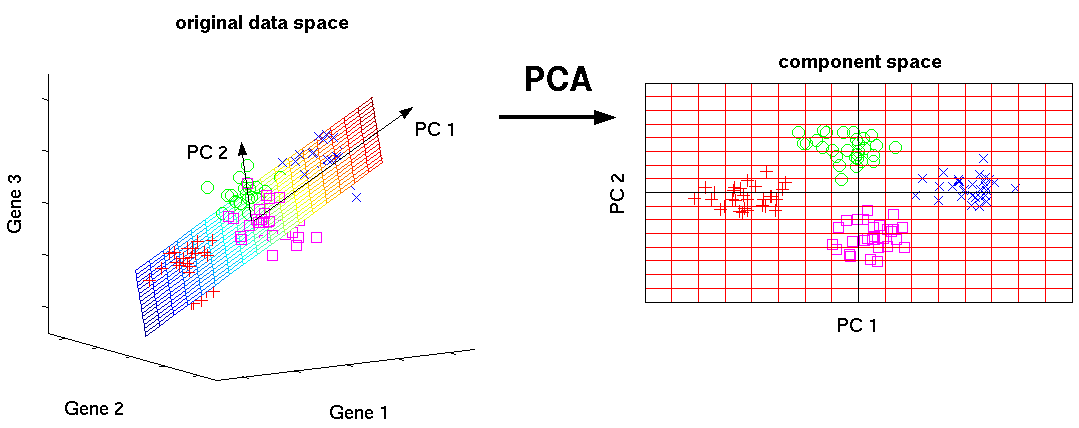
\includegraphics[width=\textwidth]{pca.png}
    \caption{Fonte: \cite{scholz2006approaches}}
    \centering
  \end{figure}
\end{frame}

\begin{frame}{Problema}

  \begin{table}
    \centering
    \begin{tabular}{ |c|c|c|c|c|c| }
    \hline
    & $x_1$ & $x_2$ & $\cdots$ & $x_{n-1}$ & $x_{n}$ \\ 
    \hline
    1 & & & & & \\ 
    \hline
    2 & & & & & \\ 
    \hline
    $\vdots$ & & & & & \\ 
    \hline
    m & & & & & \\ 
    \hline
    \end{tabular}
    \caption{Tabela com $n$ características e $m$ observações}
  \end{table}

  \begin{itemize}
    \item Como escolher os componentes (características) mais importantes?
  \end{itemize}

\end{frame}

\begin{frame}{Variância}
  \[ \sigma^2 = \frac{1}{n-1} \vt{x} \trans{\vt{x}} \]
  onde $n = \norm{\vt{x}}$.
\end{frame}

\begin{frame}{Covariância}
  \begin{defn}{Variáveis aleatórias em vetores coluna:}
    \[ \cov{x}{y} = \exptd{(\vt{x} - \exptd{\vt{x}}) \trans{(\vt{y} - \exptd{\vt{y}})}} \]

    \begin{align*}
      \cov{x}{x} &= \exptd{(\vt{x} - \exptd{\vt{x}}) \trans{(\vt{x} - \exptd{\vt{x}})}}\\
      &= \exptd{\vt{x} \trans{\vt{x}}}
    \end{align*}
  \end{defn}
\end{frame}

\begin{frame}{Covariância}

\end{frame}


\section{Regressão Linear}

\begin{frame}{Regressão Linear}
  \begin{block}{Problema:}
    \begin{itemize}
      \item Dados $n$ inputs e $n$ outputs, $(x,y)$, aproximar $f(x) = y$.
      \item Encontrar $w_0$, $w_1$ de forma que o erro em $\hat{f}(x) = w_1 x + w_0$ seja aceitável.
    \end{itemize}
  \end{block}

  \begin{figure}[t]
    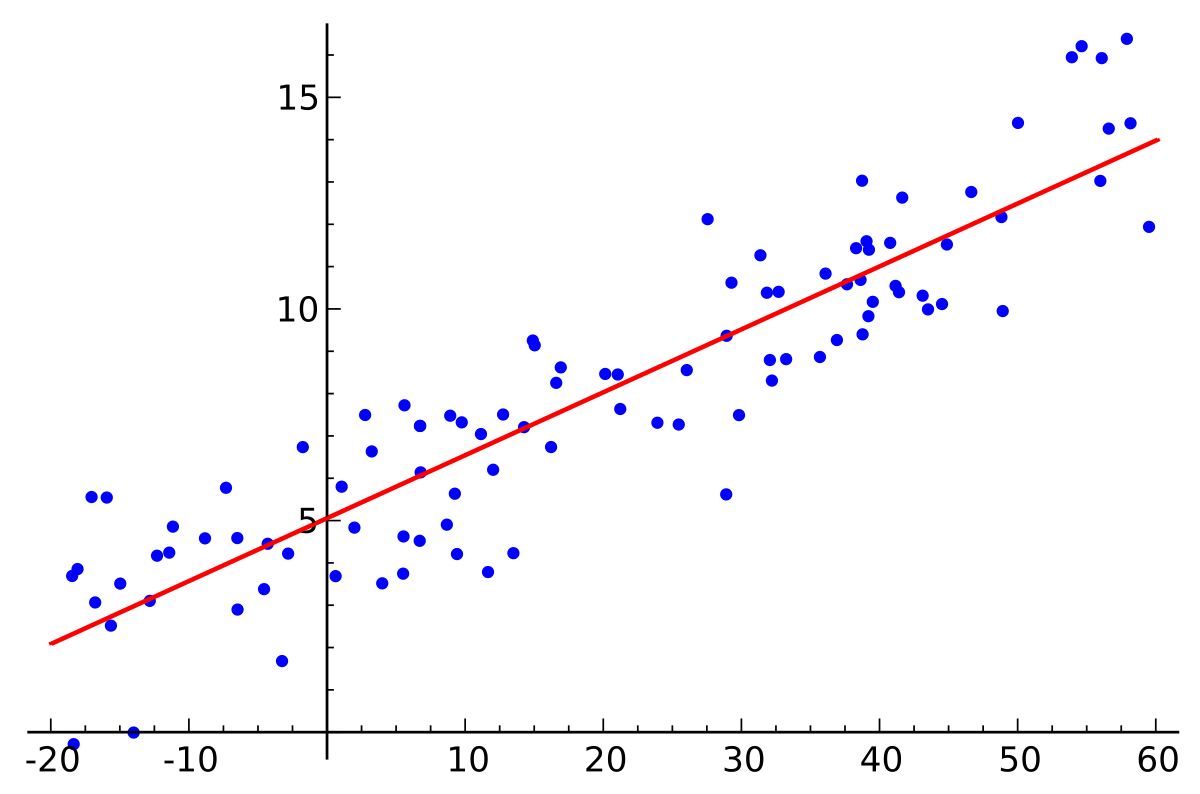
\includegraphics[width=0.5\textwidth]{lr.png}
    \centering
  \end{figure}

\end{frame}

\begin{frame}{Regressão Linear}
  \[ E(w_0, w_1 \mid x) = \frac{1}{2} \sum_{i=1}^{n} \left[y_i - (w_1 x_i + w_0)^2 \right] \]

  Para encontrar $w_0$ e $w_1$ que minizam $E$:

  \[ \frac{\partial E}{\partial w_0} = 0 \qquad \frac{\partial E}{\partial w_1} = 0 \]

  Simplificando:

  \begin{align*}
    \sum_{i=1}^{n} y_i &= n w_0 + w_1 \sum_{i=1}^{n} x_i\\
    \sum_{i=1}^{n} y_i x_i &= w_0 \sum_{i=1}^{n} x_i + w_1 \sum_{i=1}^{n} x_i^2
  \end{align*}
\end{frame}

\begin{frame}{Regressão Linear}

  \begin{align*}
    \sum_{i=1}^{n} y_i &= n w_0 + w_1 \sum_{i=1}^{n} x_i\\
    \sum_{i=1}^{n} y_i x_i &= w_0 \sum_{i=1}^{n} x_i + w_1 \sum_{i=1}^{n} x_i^2
  \end{align*}

  \begin{align*}
    A &= \begin{bmatrix}
      n & \sum x_i \\
      \sum x_i & \sum x_i^2
    \end{bmatrix} \qquad \vt{b} = \begin{bmatrix} w_0 \\ w_1 \end{bmatrix} \\
    \vt{y} &= \begin{bmatrix} \sum y_i \\ \sum y_i x_i \end{bmatrix} \quad A \vt{w} = y
  \end{align*}

  Ou seja, $ \vt{w} = A^{-1} \vt {y} $.
\end{frame}


\section{Perceptrons \& MLP}

\begin{frame}{O Modelo de McCullogh e Pitts}

  \begin{figure}[t]
    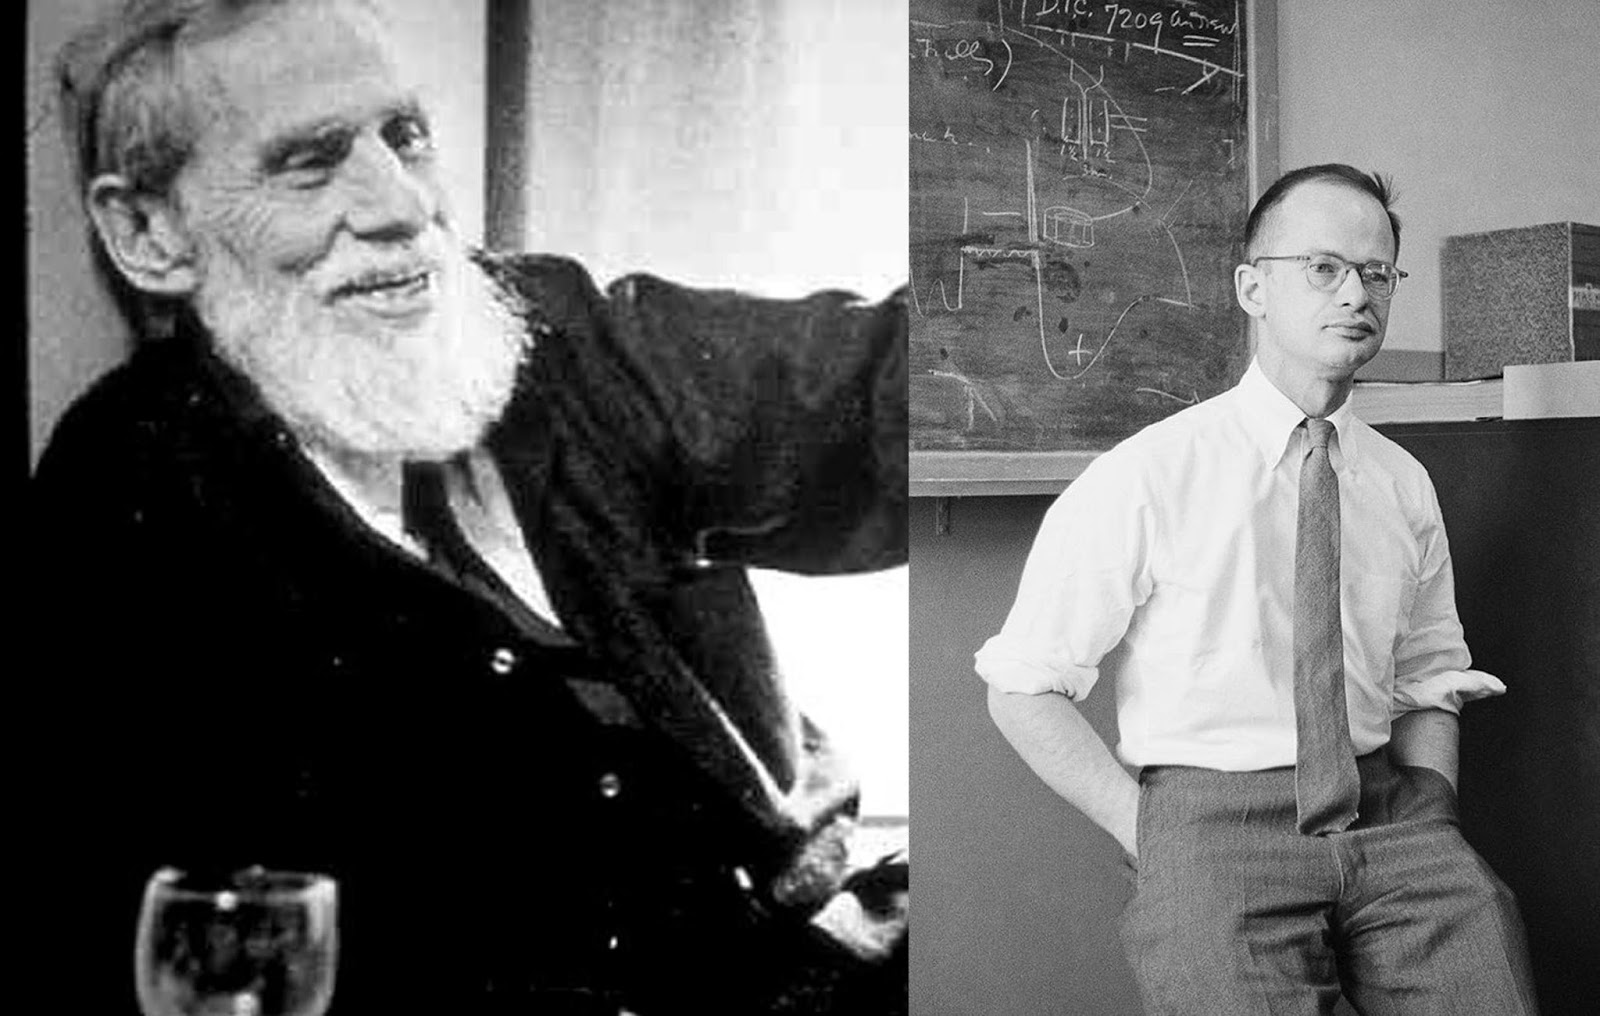
\includegraphics[width=0.8\textwidth]{warren_pitts.jpeg}
    \centering
  \end{figure}

\end{frame}

\begin{frame}{O Modelo de McCullogh e Pitts}

  \begin{figure}[t]
    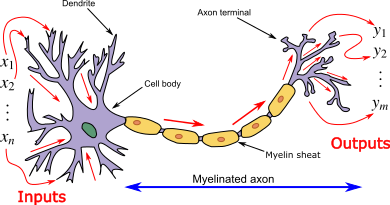
\includegraphics[width=0.8\textwidth]{neuron3.png}
    \caption{Neurônio biológico}
    \centering
  \end{figure}

\end{frame}

\begin{frame}{O Modelo de McCullogh e Pitts}

  \begin{figure}[t]
    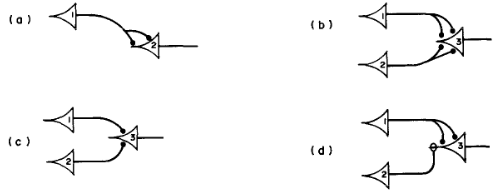
\includegraphics[width=\textwidth]{neuron1.png}
    \caption{Fonte: \cite{mcculloch1943logical}}
    \centering
  \end{figure}

\end{frame}

\begin{frame}{Aprendizado de Hebb}

  Quando um neurônio $x_i$ repetidamente ativa um neurônio $y$ a
  conexão entre $x_i$ e $y$ fica mais forte:

  \[ w_{i} = w_{i} + \eta x_i y \]

  \pause

  \begin{itemize}
    \item Conexões fortes apenas se reforçam (os pesos nunca se reduzem).
    \item Não existe noção de \"competição\" ou de limites pro aprendizado.
  \end{itemize}

\end{frame}

\begin{frame}{Aprendizado de Hebb (Generalizado)}

  \[ w_{ij} = w_{ij} + \eta y_j \left(x_i - \sum_{k=1}^{j} w_{ik}y_{k} \right)\]

  Um input é distribuido de forma incremental nos múltiplos outputs.

\end{frame}

\begin{frame}{Perceptron - Rosenblatt}

  \begin{figure}
    \begin{tikzpicture}
      \node[functions] (center) {};
      \node[below of=center,font=\scriptsize,text width=4em] (threshold) {Função de Ativação};
      \draw[thick] (0.5em,0.5em) -- (0,0.5em) -- (0,-0.5em) -- (-0.5em,-0.5em);
      \node[output, right=1.5em of center] (Y) {Y};
      \draw (0em,0.75em) -- (0em,-0.75em);
      \draw (0.75em,0em) -- (-0.75em,0em);
      \node[right of=center] (right) {};
        \path[draw,->] (center) -- (right);
      \node[functions,left=3em of center] (left) {$\sum$};
        \path[draw,->] (left) -- (center);
      \node[weights,left=3em of left] (2) {$w_2$} -- (2) node[input,left of=2] (l2) {$x_2$};
        \path[draw,->] (l2) -- (2);
        \path[draw,->] (2) -- (left);
      \node[below of=2] (dots) {$\vdots$} -- (dots) node[left of=dots] (ldots) {$\vdots$};
      \node[weights,below of=dots] (n) {$w_n$} -- (n) node[input,left of=n] (ln) {$x_n$};
        \path[draw,->] (ln) -- (n);
        \path[draw,->] (n) -- (left);
      \node[weights,above of=2] (1) {$w_1$} -- (1) node[input,left of=1] (l1) {$x_1$};
        \path[draw,->] (l1) -- (1);
        \path[draw,->] (1) -- (left);
      \node[weights,above of=1,fill=red!150!green!10] (0) {$w_0$} -- (0) node[input,left of=0,fill=red!150!green!10] (l0) {$x_0$};
        \path[draw,->] (l0) -- (0);
        \path[draw,->] (0) -- (left);
      \node[below of=ln,font=\scriptsize] {Inputs};
      \node[below of=n,font=\scriptsize] {Pesos};
    \end{tikzpicture}
  \centering
  \end{figure}

\begin{align}
Y = \left\{
  \begin{array}{cc}
    1 & \text{ se } \sum_{i=0}^{n} w_i x_i - T > 0 \\
    0 & \text{ caso contrário } \\
  \end{array} \right.
\end{align}

\end{frame}

\begin{frame}{Perceptron (1958) - Ajustando os pesos}

Seja $m$ o número de iterações.
\begin{align*}
  S(m) &= \sum_{i=0}^{n} w_i^m x_i^m \\
       &= \trans{\vt{w}}_m \vt{x}_m
\end{align*}

\begin{itemize}
  \item Se $\vt{x}_m$ é classificado de forma correta:
    \[ \vt{w}_{m+1} = \vt{w}_m \]
  \item Caso contrário, seja $\eta(m)$ uma taxa de aprendizado variando em $m$:
    \[ \vt{w}_{m+1} = \vt{w}_m - \eta(m) \vt{x}_m \]
\end{itemize}


\end{frame}

\begin{frame}{Perceptron (1958) - F.Rosenblatt}
  Consegue aprender:
  \begin{itemize}
    \item Funções booleanas.
    \item Atualiza os pesos quando encontra uma resposta errada.
    \item Rosenblatt provou formalmente que o algoritmo converge para problemas linearmente separáveis.
  \end{itemize}
\end{frame}

\begin{frame}{Perceptron - Rosenblatt}

  \begin{figure}
    \begin{tikzpicture}
    \node [input] (A) at (0,0)  {X};
    \node [input] (B) at (0,-2) {Y};
    \node [input] (C) at (3,-1) {1};
    \node [output, scale=0.5] (D) at (4.5,-1) {X $\lor$ Y};
    \path (A) edge node[above]{1} (C);
    \path (B) edge node[above]{1} (C);
    \path[draw, ->] (C) -- (D);
    \end{tikzpicture}
  \centering
  \end{figure}

  \begin{figure}
    \begin{tikzpicture}
    \node [input] (A) at (0,0)  {X};
    \node [input] (B) at (0,-2) {Y};
    \node [input] (C) at (3,-1) {2};
    \node [output, scale=0.5] (D) at (4.5,-1) {X $\land$ Y};
    \path (A) edge node[above]{1} (C);
    \path (B) edge node[above]{1} (C);
    \path[draw, ->] (C) -- (D);
    \end{tikzpicture}
  \centering
  \end{figure}

\end{frame}

\begin{frame}{Perceptron (1958) - F.Rosenblatt}
  \begin{block}{The New York Times (1958) \cite{olazaran1996sociological}}
    The Navy revealed the embryo of an electronic computer today that it expects will be able to walk, talk, see, write, reproduce itself and be conscious of its existence. Later perceptrons will be able to recognize people and call out their names and instantly translate speech in one language to speech and writing in another language, it was predicted.
  \end{block}
\end{frame}

\begin{frame}{Perceptrons (1969) - Minsky \& Papert}

  \begin{figure}
    \begin{tikzpicture}
    \node [input] (A) at (0,0)  {X};
    \node [input] (B) at (0,-2) {Y};
    \node [input] (C) at (3,-1) {?};
    \node [output, scale=0.5] (D) at (4.5,-1) {X $\oplus$ Y};
    \path (A) edge node[above]{?} (C);
    \path (B) edge node[above]{?} (C);
    \path[draw, ->] (C) -- (D);
    \end{tikzpicture}
  \centering
  \end{figure}

\end{frame}

\begin{frame}{Perceptrons (1969) - Minsky \& Papert}

  \begin{figure}
    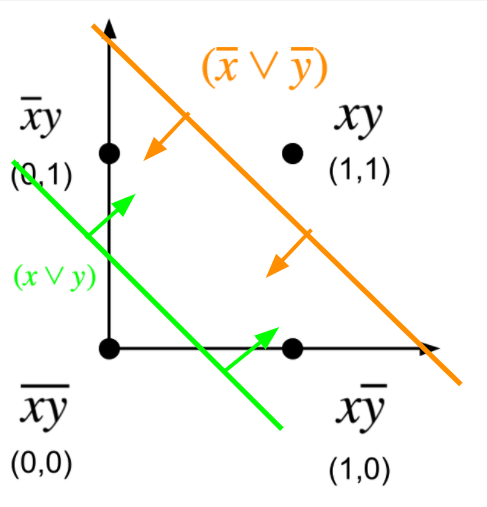
\includegraphics[width=0.55\linewidth]{minsky2.png}
  \end{figure}

  \begin{itemize}
    \item A Pesquisa sobre Perceptrons entrou em declínio em 1969, quando Marvin Minsky e Seymour Papert publicaram o livro "Perceptrons", onde eles descreveram algumas limitações do modelo.
  \end{itemize}

\end{frame}

\begin{frame}{Multi-Layer Perceptrons (1969) - Minsky \& Papert}

  \begin{figure}
    \begin{tikzpicture}
    \node [input] (A) at (0,0)  {X};
    \node [input] (B) at (0,-2) {Y};
    \node [input] (C) at (3,0)  {};
    \node [input] (D) at (3,-2) {};
    \node [output, scale=0.5] (E) at (5,-1) {X $\oplus$ Y};
    \path (A) edge node[above]{?} (C);
    \path (A) edge node[above]{?} (D);
    \path (B) edge node[below]{?} (C);
    \path (B) edge node[above]{?} (D);
    \path[draw, ->] (C) -- (E);
    \path[draw, ->] (D) -- (E);
    \end{tikzpicture}
  \centering
  \end{figure}

\end{frame}

\begin{frame}{MLP - Backpropagation}

\begin{figure}[t]
  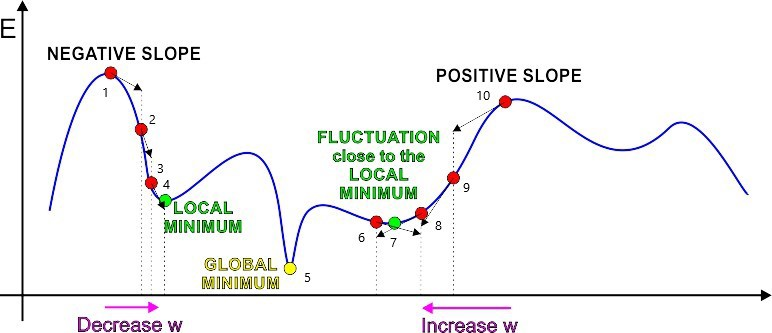
\includegraphics[width=0.7\textwidth]{gd.jpeg}
  \caption{O próximo passo deve ser tomado de forma a diminuir o erro $E$ em nossa rede. Uma boa opção é seguir a direção oposta ao gradiente de $E$.}
  \centering
\end{figure}

Seja $n$ o número de iterações e $W$ a matriz de pesos da rede, temos que:
\begin{align*}
  W^{(n+1)}_{ji} = W^{(n)}_{ji} + \Delta W^{(n)}_{ji}
\end{align*}

\end{frame}

\begin{frame}{MLP - Backpropagation}

Seja $n$ o número de iterações e $W$ a matriz de pesos da rede, temos que:
\[ W^{(n+1)}_{ji} = W^{(n)}_{ji} + \Delta W^{(n)}_{ji} \]
onde:
\[ \Delta W^{(n)}_{ji} = -\eta \frac{\partial E}{\partial W_{ji}} \]
e $\eta \in [0, 1]$.

\end{frame}

\begin{frame}{MLP - Backpropagation}

\[ \frac{\partial E}{\partial W_{ji}} = \frac{\partial E}{\partial V_j} \frac{\partial V_j}{\partial W_{ji}} \]
\[ \delta_j = - \frac{\partial E}{\partial V_j} \qquad y_i = \frac{\partial V_j}{\partial W_{ji}} \]
\[ \Delta W^n_{ji} = \eta \delta^n_j y^n_i \]

\begin{block}{Regra-$\Delta$:}
\[
  \delta_j =
    \begin{cases}
      f^\prime(V_j)(y^\ast_j - y_i) \text{ se $j$ é um neurônio de output}\\
      f^\prime(V_j)(\sum_{k} \delta_k W_{jk}) \text{ se $j$ é um neurônio escondido}
    \end{cases}
\]
\end{block}

\end{frame}

\begin{frame}{The Universal Approximation Theorem}
  \begin{figure}[t]
    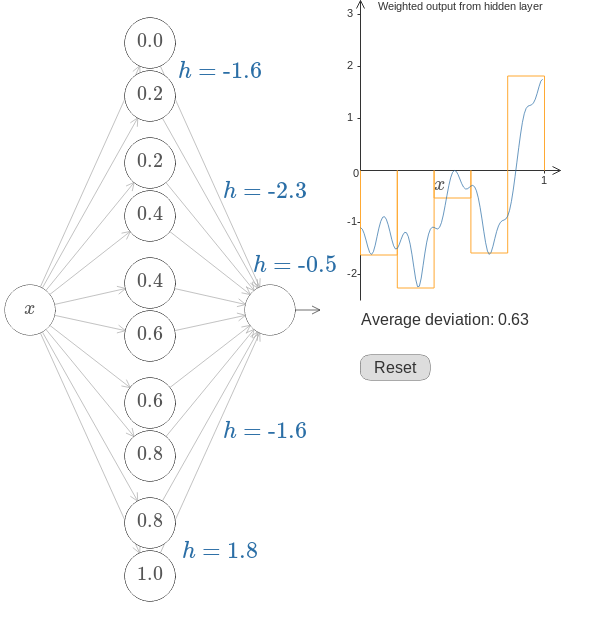
\includegraphics[width=0.7\textwidth]{uat00.png}
    \centering
  \end{figure}
\end{frame}

\section{Validando Experimentos}

\begin{frame}{Problema}
  \begin{itemize}
    \item Qual a diferença entre aprender e decorar?
    \item O experimento está convergindo?
    \item Como saber se o algoritmo realmente generalizou um problema?
  \end{itemize}
\end{frame}

\begin{frame}{Problema}
  \[ \sum_{x_t \in X} (x_t - x_{t}^d) = \varepsilon \]
\end{frame}

\begin{frame}{Validação}
  \begin{block}{Como saber se o algoritmo realmente generalizou um problema?}
  Quando ele consegue se sair bem em dados ainda não vistos.
  \end{block}

  \pause

  \begin{itemize}
    \item Separe uma parte dos dados para teste.
    \item Separe uma parte dos dados de treino para validar o próprio treinamento.
  \end{itemize}

  \begin{figure}[t]
    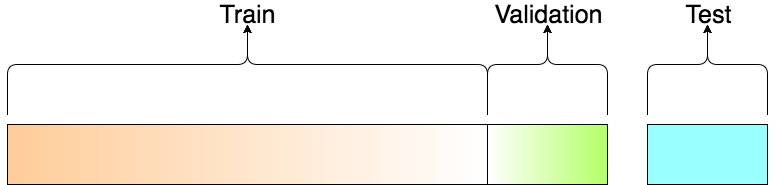
\includegraphics[width=\textwidth]{validation.png}
    \centering
  \end{figure}

\end{frame}

\begin{frame}{Validação Cruzada (K-Fold CV)}
  \begin{block}{Problemas com o método anterior}
    \begin{itemize}
      \item A escolha dos dados pra validação depende muita de sorte.
    \end{itemize}
  \end{block}

  \pause

  \begin{figure}[t]
    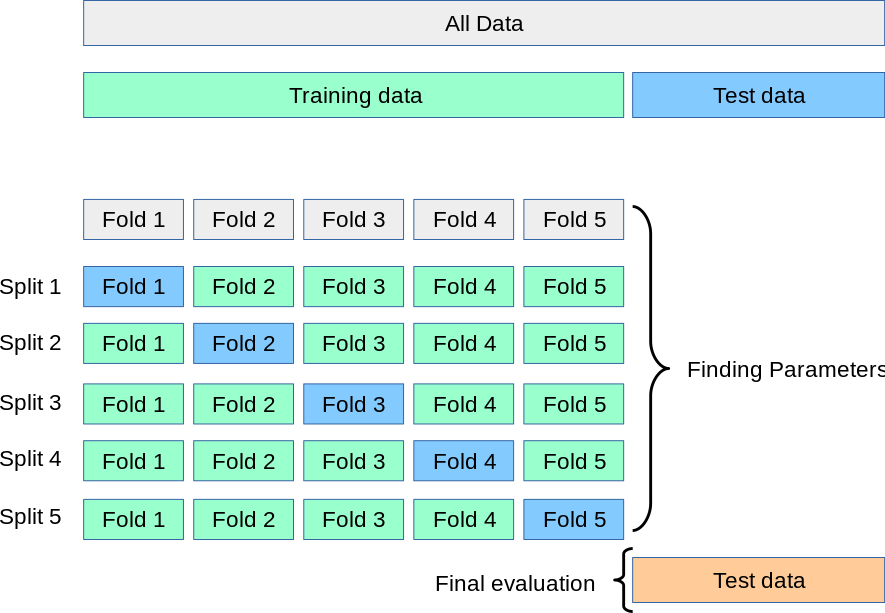
\includegraphics[width=0.6\textwidth]{cross_validation.png}
    \caption{5-Fold cross validation, Fonte: \href{https://scikit-learn.org/stable/modules/cross_validation.html}{scikit-learn}.}
    \centering
  \end{figure}

\end{frame}

\begin{frame}{Monte Carlo cross-validation}
  \begin{figure}[t]
    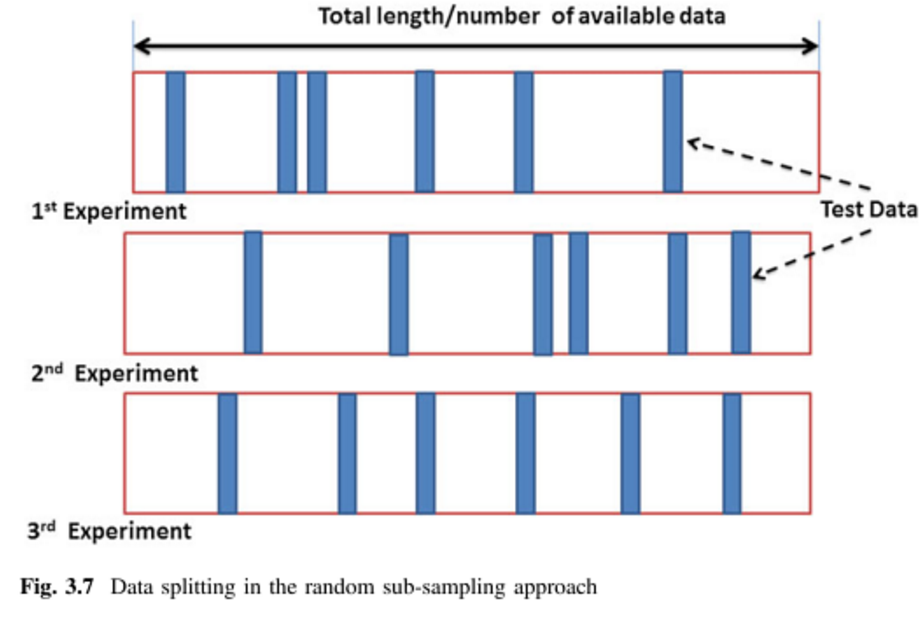
\includegraphics[width=0.8\textwidth]{monte_carlo.png}
    \centering
  \end{figure}
\end{frame}

\begin{frame}{Overfitting}

  \begin{figure}[t]
    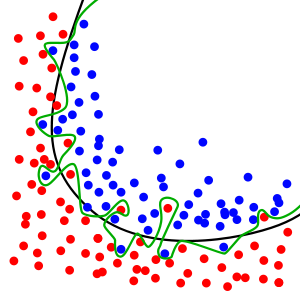
\includegraphics[width=0.6\textwidth]{overfitting.png}
    \caption{Fonte: \href{https://en.wikipedia.org/wiki/Overfitting}{Wikipedia}.}
    \centering
  \end{figure}

\end{frame}

\begin{frame}{Regularização}

\begin{block}{}
  \[ \min \left(\sum_{x_t \in X} (x^\ast_t - x^d_t) + \norm{P} \right) \]
\end{block}

\end{frame}


% END
%--------------------------------------

{\setbeamercolor{palette primary}{fg=black, bg=yellow}
\begin{frame}[standout]
  Perguntas?
\end{frame}
}

\begin{frame}{Créditos:}

  Baseado nos materiais de:
  \begin{itemize}
    \item \href{http://deeplearning.cs.cmu.edu/}{http://deeplearning.cs.cmu.edu}
  \end{itemize}

\end{frame}


\begin{frame}[allowframebreaks]{Referências}

  \bibliography{references}
  \bibliographystyle{apalike}

\end{frame}

\end{document}
